\section{Phase two} %This is where we examine if we can classify correctly
In evaluating the generated map, our aim is to determine if the system can accurately distinguish whether a receiving device is situated inside or outside the room.
\begin{figure}[h]
    \centering
    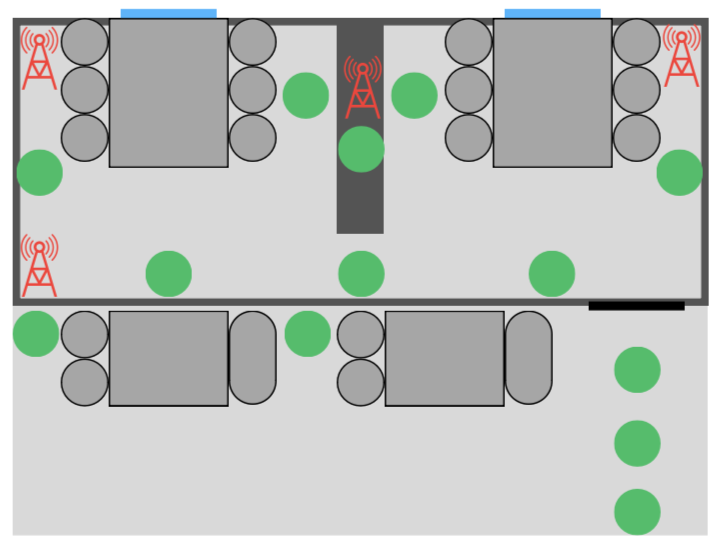
\includegraphics[scale=0.5]{images/experiment_setup.png}
    \caption{A sketch of the meeting room in which the experiments were carried out, decorated with beacon placements (red antenna) and measurement locations(green circles)}
    \label{fig:experiment_setup}
\end{figure}
As described in Section \ref{sec:bluetooth_low_energy}, physical obstacles can cause fluctuations in the received signals. 
Therefore, we design the expirement such that measurements are taken in areas where some, none, and all of the beacons are blocked. 
We perform measurements in the following areas:
\begin{itemize}
    \item Along the walls inside of the meeting room, to examine border values of the map while inside the room
    \item Along both sides of the divider, to examine whether obstructions inside the room has any meaningful effect on the classification
    \item On the cabinet, next to the beacon, to examine classification of a receiver placed in the middle of the room
    \item $1$ meter, $2$ meters, and $3$ meters outside the door, to examine how far away from the meeting a receiver must be before it is classified as outside.
    \item By the tables in the common area, to ensure that we do not classify an outside area as an inside area.
\end{itemize}
For each of these areas 10 data points has been collected and classified on several devices.
Data collection points and beacon placement of the room during the experiment is shown in Figure \ref{fig:experiment_setup}. 